\documentclass[a4paper,11pt]{article}
\usepackage[utf8]{inputenc}
\usepackage[T1]{fontenc}
\usepackage[french]{babel}
\usepackage{makeidx}
\usepackage{textcomp}
\usepackage{graphicx}
\usepackage{mathtools,amssymb,amsthm}
\usepackage{lmodern}
\usepackage{multirow}
\usepackage{array}
\usepackage{longtable}

\title{TER 2019 - Spécifications}
\author{Maxime Gonthier - Benjamin Guillot - Laureline Martin}
\begin{document}
	\pagenumbering{gobble}\clearpage
	\maketitle

\newpage
\tableofcontents

\newpage
\section{Introduction}
Ce rapport à pour objectif de décrire dans un premier temps les données que nous allons utiliser dans notre projet et nous détaillerons les étapes à suivre pour exploiter ces données. Ensuite nous expliquerons le calcul de la congestion. Enfin nous expliquerons la stratégie d'optimisations que nous utiliserons. Tous cela sera explicité sous la forme d'un exemple simple.

\section{Les données initiales}
	\subsection{La courbe de trafic}
		La courbe de trafic est le nombre de personnes qui montent et descendent du bus à chaque arrêt. Dans notre cas d'étude, c'est à dire l'université, nous considérons que tous les étudiants montent au premier arrêt (une gare) et descendent au terminus (l'université). La courbe de trafic ajoute des montées et des descentes à chaque arrêt, ce sont des non-étudiants. \\
		On considère qu'il y a un bus partant de la gare tout les quart d'heure, le temps étant représenté par tranche de 15 minutes dans notre application.\\
		Dans notre exemple nous avons : \\
		\begin{tabular}{ | c | c | c | c | c | c |}
 			\hline			
   			Numéro de l'arrêt & 1 & 2 & 3 & 4 & 5\\
   			Montées & 50 & 15 & 10 & 2 & 0 \\
   			Descentes & 0 & 5 & 10 & 8 & 54\\
 			\hline  
 		\end{tabular}\\
 		La valeur de montée du premier arrêt est choisis arbitrairement et la valeur de descente du terminus considère que tous le monde descend à cet arrêt, pour plus de simplicité. 
 		Pour obtenir les données des arrêts intermédiaires nous choisirons une valeur aléatoire, choisis dans un intervalle différent en fonction de l'heure, l'objectif est de représenter la congestion forte des heures de pointes de manière un peu plus précise : \\
 		\begin{tabular}{ | c | c | c | c | c | c |}
 			\hline			
   			Horaire & 7-8h & 8-9h & 9-10h & 10-11h & 11-12h\\
   			Montées & [5:10] & [5:10] & [3:10] & [2:8] & [1:5] \\
   			Descentes & [0:5] & [0:5] & [1:6] & [1:6] & [1:5]\\
 			\hline  
 		\end{tabular}\\

	\subsection{L'emploi du temps}
		L'emploi du temps est un graphe dont les sommets sont des cours et les liens des contraintes entre les cours. Les contraintes seront déterminé par une matrice d'adjacence.
		Pour plus de clarté nous considérons ici que chaque professeur est disponible sur toute la durée de la journée.
		Dans notre exemple nous nous limitons à 10 sommets.
		\begin{enumerate}
			\item On créer un graphe non orienté en numérotant les sommets de 1 à 10.
			\centerline{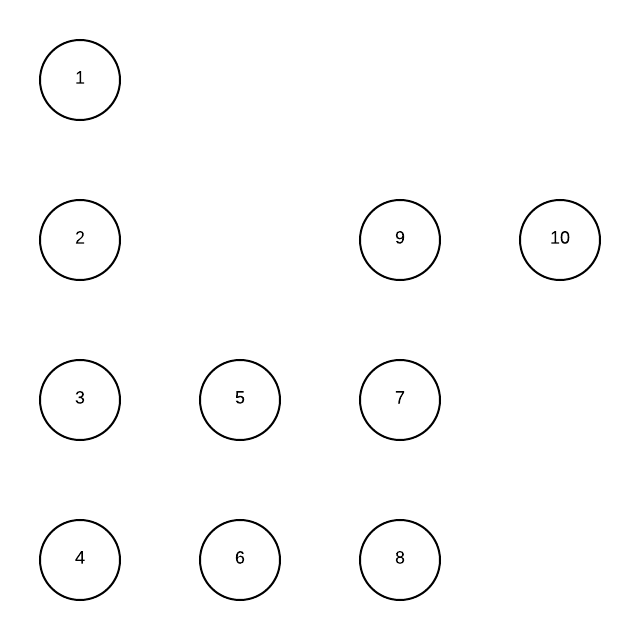
\includegraphics[scale=0.8]{Captures/exemple1.png}}
			\item On relie les sommets entre eux lorsque qu'il y a une contrainte (même étudiant sur des horaires qui se chevauchent). Pour cela on créé une matrice d'adjacence avec un degré moyen choisis arbitrairement. Pour N sommets et K le degré moyen, la probabilité qu'il y ai une arête à insérer dans chaque case est K/N.
			\item On oriente les arêtes désormais des sommets de degrés le plus faible au plus fort.\\
			\centerline{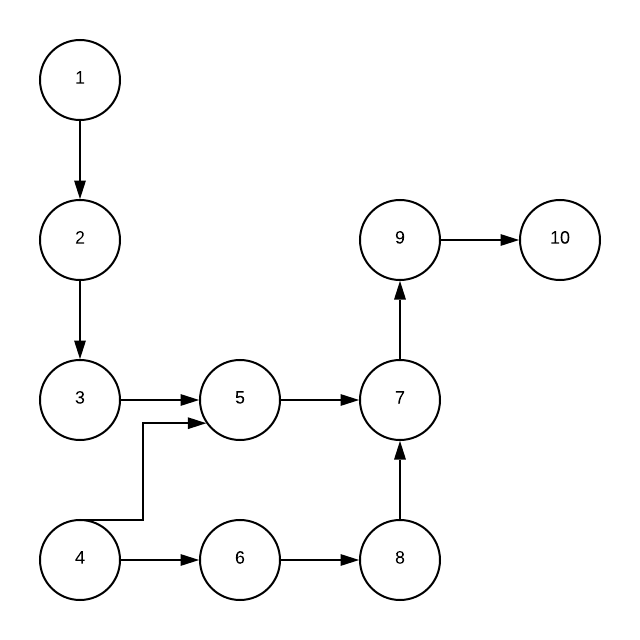
\includegraphics[scale=0.8]{Captures/exemple2.png}}
			\item On remarque dans notre exemple qu'il y a deux sommets de degré entrant nul, ces deux sommets de notre DAG seront des points de départs possible pour notre planification.
			\item On colorie le graphe, chaque couleur représente une salle.\\
			\centerline{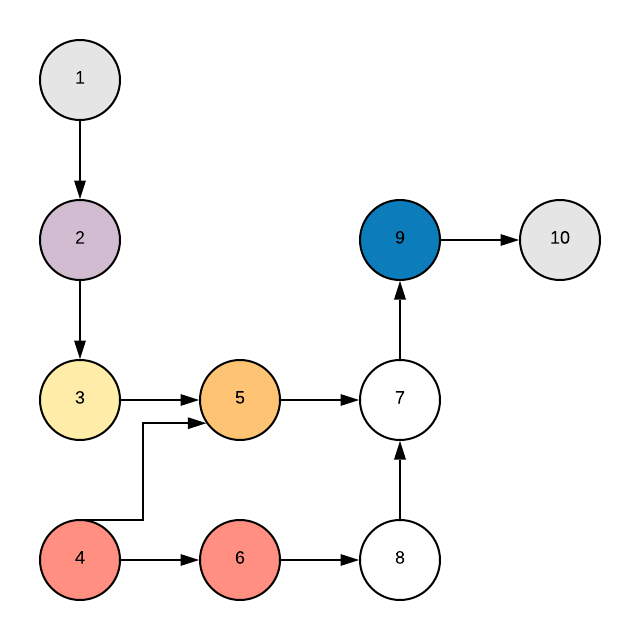
\includegraphics[scale=0.8]{Captures/exemple3.png}}
			\item Nous agençons l'emploi du temps en respectant le fait que deux couleurs et deux sommets reliés par un arc ne peuvent pas être sur la même plage horaire. Par défaut le sommet duquel nous partirons est le sommet de degré entrant nul le plus faible, ici le numéro 1.
			\centerline{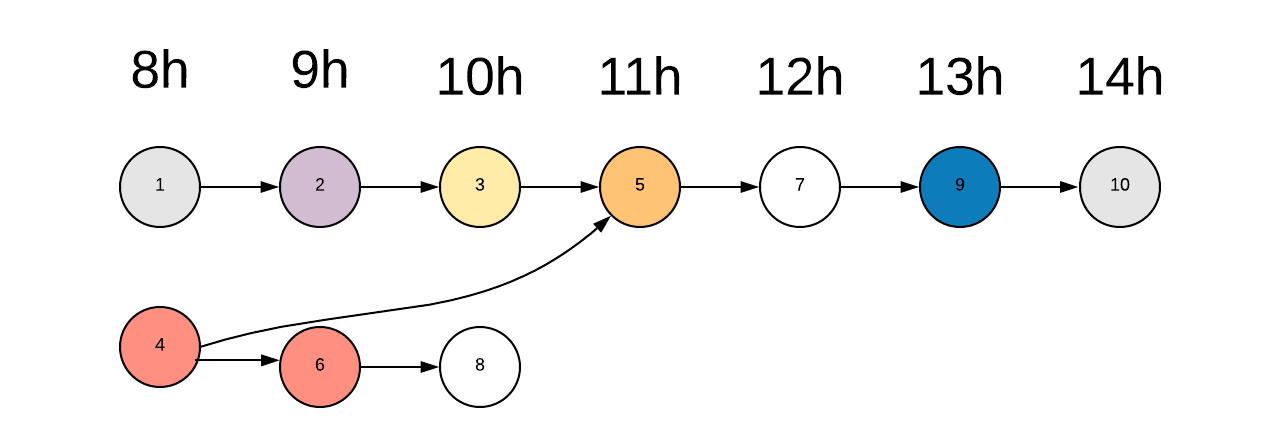
\includegraphics[scale=0.8]{Captures/exemple4.png}}
		\end{enumerate}
		Chaque cours possède un nombre d'étudiants choisis aléatoirement entre 16 et 32 pour un TD et entre 16 et 100 pour un cours magistral. les TDs représentent trois quart des cours. Ainsi dans notre exemple nous avons : \\
		\begin{tabular}{ | c | c | c | c | c | c | c | c | c | c | c |}
 			\hline			
   			Numéro du sommet & 1 & 2 & 3 & 4 & 5 & 6 & 7 & 8 & 9 & 10\\
   			Type de cour & TD & CM & CM & TD & TD & TD & TD & TD & TD & CM \\
   			Nombre d'élèves & 16 & 70 & 60 & 30 & 25 & 20 & 16 & 30 & 14 & 50\\
 			\hline  
 		\end{tabular}\\

\section{Calcul de congestion}
	A l'aide du tableau ci dessus nous allons pouvoir déterminé à chaque horaire le nombre d'étudiants arrivé au terminus et donc en conclure à l'aide du tableau des montées et des descentes le nombre de personnes à chaque arrêt. 
	On considère que les etudiants prennent le bus arrivant 15 min avant leurs premier cour de la journée.
	Dans notre exemple nous avons pour  8h le cours 1 et 4, ce qui représente 46 élèves. Ainsi le bus de arrivant a 7h45 ressemble à cela :  \\
	\begin{tabular}{ | c | c | c | c | c | c | c |}
 			\hline			
   			Numéro de l'arrêt & 1 & 2 & 3 & 4 & 5\\
   			Différence montées/descentes & 10 & 7 & 10 & 11 & 0\\
   			Nombre de personnes dans le bus & 56 & 53 & 60 & 56 & 57\\
 			\hline  
 	\end{tabular}\\
 	Ce tableau sera générés pour chaque bus. On mesurera dans chaque cas le dépassement à chaque arrêt en mettant un 1 si il y a dépassements, un 0 sinon.
 	Sachant que la limite de confort est de 50 dans le bus que nous étudions, ce bus nous donne une valeur de congestion de 5.
 	Il faudra pour les bus suivants prendre en compte les élèves déjà présent à l'université avant de calculer le nombre de personnes dans le bus.

\section{Stratégie d'optimisation}
	\subsection{Mise en rapport de la congestion et des sommets}
		Il faut dans un premier temps déterminer quels sommets sont les plus impactant en terme de congestion. Une manière de les trier peut être par ordre décroissant de leurs nombre d'étudiants. Ensuite on rechercherais une solution gloutonne où les sommets ayant le plus d'étudiants ont lieu à des horaires où les autres cours ont peu d'étudiants, c'est à dire que nous allons minimiser la somme des étudiants ayant cours au même moments. Évidemment le point de départ sera toujours un sommet de degré entrant nul. Dans notre exemple on aurait pour le tri : \\
		\begin{tabular}{ | c | c | c | c | c | c | c | c | c | c | c |}
 			\hline			
   			Numéro du sommet & 2 & 3 & 10 & 4 & 8 & 5 & 6 & 7 & 1 & 9\\
   			Nombre d'élèves & 70 & 60 & 50 & 30 & 30 & 25 & 20 & 16 & 16 & 14\\
 			\hline  
 		\end{tabular}\\	
 		On place en premier le sommet 1 à 8h car il est de degré entrant nul. Ensuite on place le sommet 2 à 9h pour ne pas être en même temps que le 4. Ainsi de suite. Une fois arrivé à l'horaire limite de notre exemple (14h) on place les sommets au endroit où la somme des étudiants sera le plus faible possible. Ainsi le sommet 6 va à la même horaire que le sommet 5, le 7 à la même horaire que le 8, impossible ils ont la même couleur, donc le 7 va a la même horaire que le suivant, le 4 etc...
 		Après l'optimisation gloutonne on aura : \\
 		\centerline{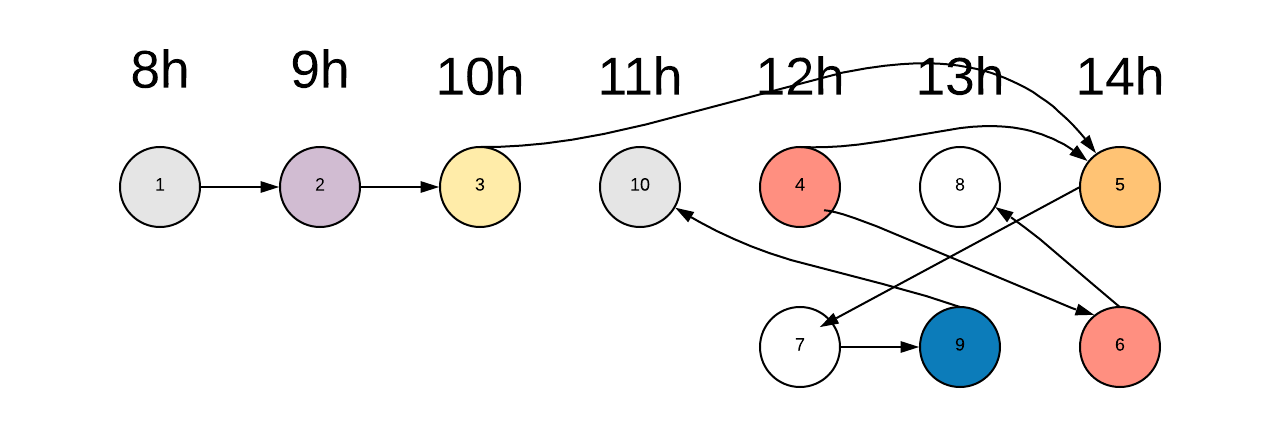
\includegraphics[scale=0.8]{Captures/exemple5.png}}\\
 		On recalcule ensuite la congestion de chaque bus comme vue précédemment.

 	\subsection{Recherche tabou}
 		A partir de la première solution obtenu grâce à l'approche gloutonne nous allons explorer le voisinage de cette dernière pour tenter de trouver des optimums locaux.\\
 		On va modifier l'horaire des cours 1 à 1 de manière aléatoire en commençant par le cours ayant le plus d'étudiant. Pour chaque solution on recalcule la congestion et on interdit la configuration pour les prochaines solutions. Dans notre exemple on va dans un premier temps bouger le sommet 2 de 9h à 10h. Ensuite on recherche la solution suivante en prenant en compte cette modification. On procède de la sorte pendant un nombre d'itérations arbitraire. En effet on ne peux pas savoir quand arrêter la simulation car on ne peux pas être sûr qu'un optimum local est aussi global.\\
 		Ensuite nous allons appliquer le même procéder mais en faisant varier les horaires de deux sommets à la fois a chaque itérations.
 		Durant l'exécution de l'application, on va potentiellement trouver un grand nombre de solution viables. On va enregistrer chaque solutions viables et leur attribuer un score. Ce score sera la somme des dépassements du seuil de confort de chaque bus. La solution retenu a la fin de l'exécution sera celle ayant le plus petit score.
\end{document}
